% !TEX root =  main.tex

\section{The Inevitable Bias of Nested Estimation} 
\label{sec:bias}

The previous section confirmed the capabilities of NMC; in this section we establish a
limitation by proving that NMC schemes must produce biased estimates of $I(f)$ for certain
functions $f$. In fact, our result applies more generally: we show that this holds for any
Monte Carlo scheme that makes use of imperfect estimates $\hat{\zeta}_n$ of $\gamma(y_n)$,
either via a nested Monte Carlo procedure (e.g. $\hat{\zeta}_n = (\hat{\gamma}_M)_n$), or
when these inner estimates are generated by some other potentially deterministic methods
such as a variational approximation~\citep{blei2016variational} or Bayesian
quadrature~\citep{o1991bayes}.
%A characterization of this result is shown in Figure~\ref{fig:bias-plot} and more formally
%in the following Theorem.
\begin{theorem}
  Suppose that the random variables $\hat{\zeta}_n$ satisfy
    $\mathbb{P}(\hat{\zeta}_n \neq \gamma(y_n)) > 0$.
  Then we can choose $f$ such that if $y_n \sim p(y)$,
    $\E\left[\frac{1}{N} \sum_{n=1}^N f(y_n, \hat{\zeta}_n)\right] \neq I(f)$ for any
    $N$ (including $N\rightarrow\infty$).
\end{theorem}
\begin{proof}
	Take $f(y, w) = (\gamma(y) - w)^2$. Then $f(y, \gamma(y)) = 0$, so that $I(f) = 0$.  On
	the other hand, $f(y_n, \hat{\zeta}_n) \geq 0$ since $f$ is non-negative.
	Moreover, $f(y_n, \hat{\zeta}_n) > 0$ on the event $\{\hat{\zeta}_n \neq \gamma(y_n)\}$.
	Since we assumed this event has nonzero probability, it follows that $\E \left[f(y_n, \hat{\zeta}_n)\right] > 0$ and hence
	\[
	\E\left[\frac{1}{N} \sum_{n=1}^N f(y_n, \hat{\zeta}_n)\right]
	= \frac{1}{N} \sum_{n=1}^N \E\left[f(y_n, \hat{\zeta}_n)\right]
	> 0 = I(f)
	\]
	which gives the required result.
\end{proof}
%\begin{remark}
%  Here $\hat{\zeta}_n$ may take the form
%  $\hat{\zeta}_n = (\hat{\gamma}_M)_n$ from \eqref{eq:nested-inner} where an NMC scheme is
%  used. However, we do not require this: apart from implicit measurability properties, our
%  assumption is only that $\hat{\zeta}_n$ is an \emph{imperfect} estimator of
%  $\gamma(y_n)$, which is by definition the case for any approximate estimation method
%  such as MC, variational approximations, or Bayesian quadrature~\cite{o1991bayes}.
%\end{remark}
%
%
%\begin{figure}
%	\centering
%	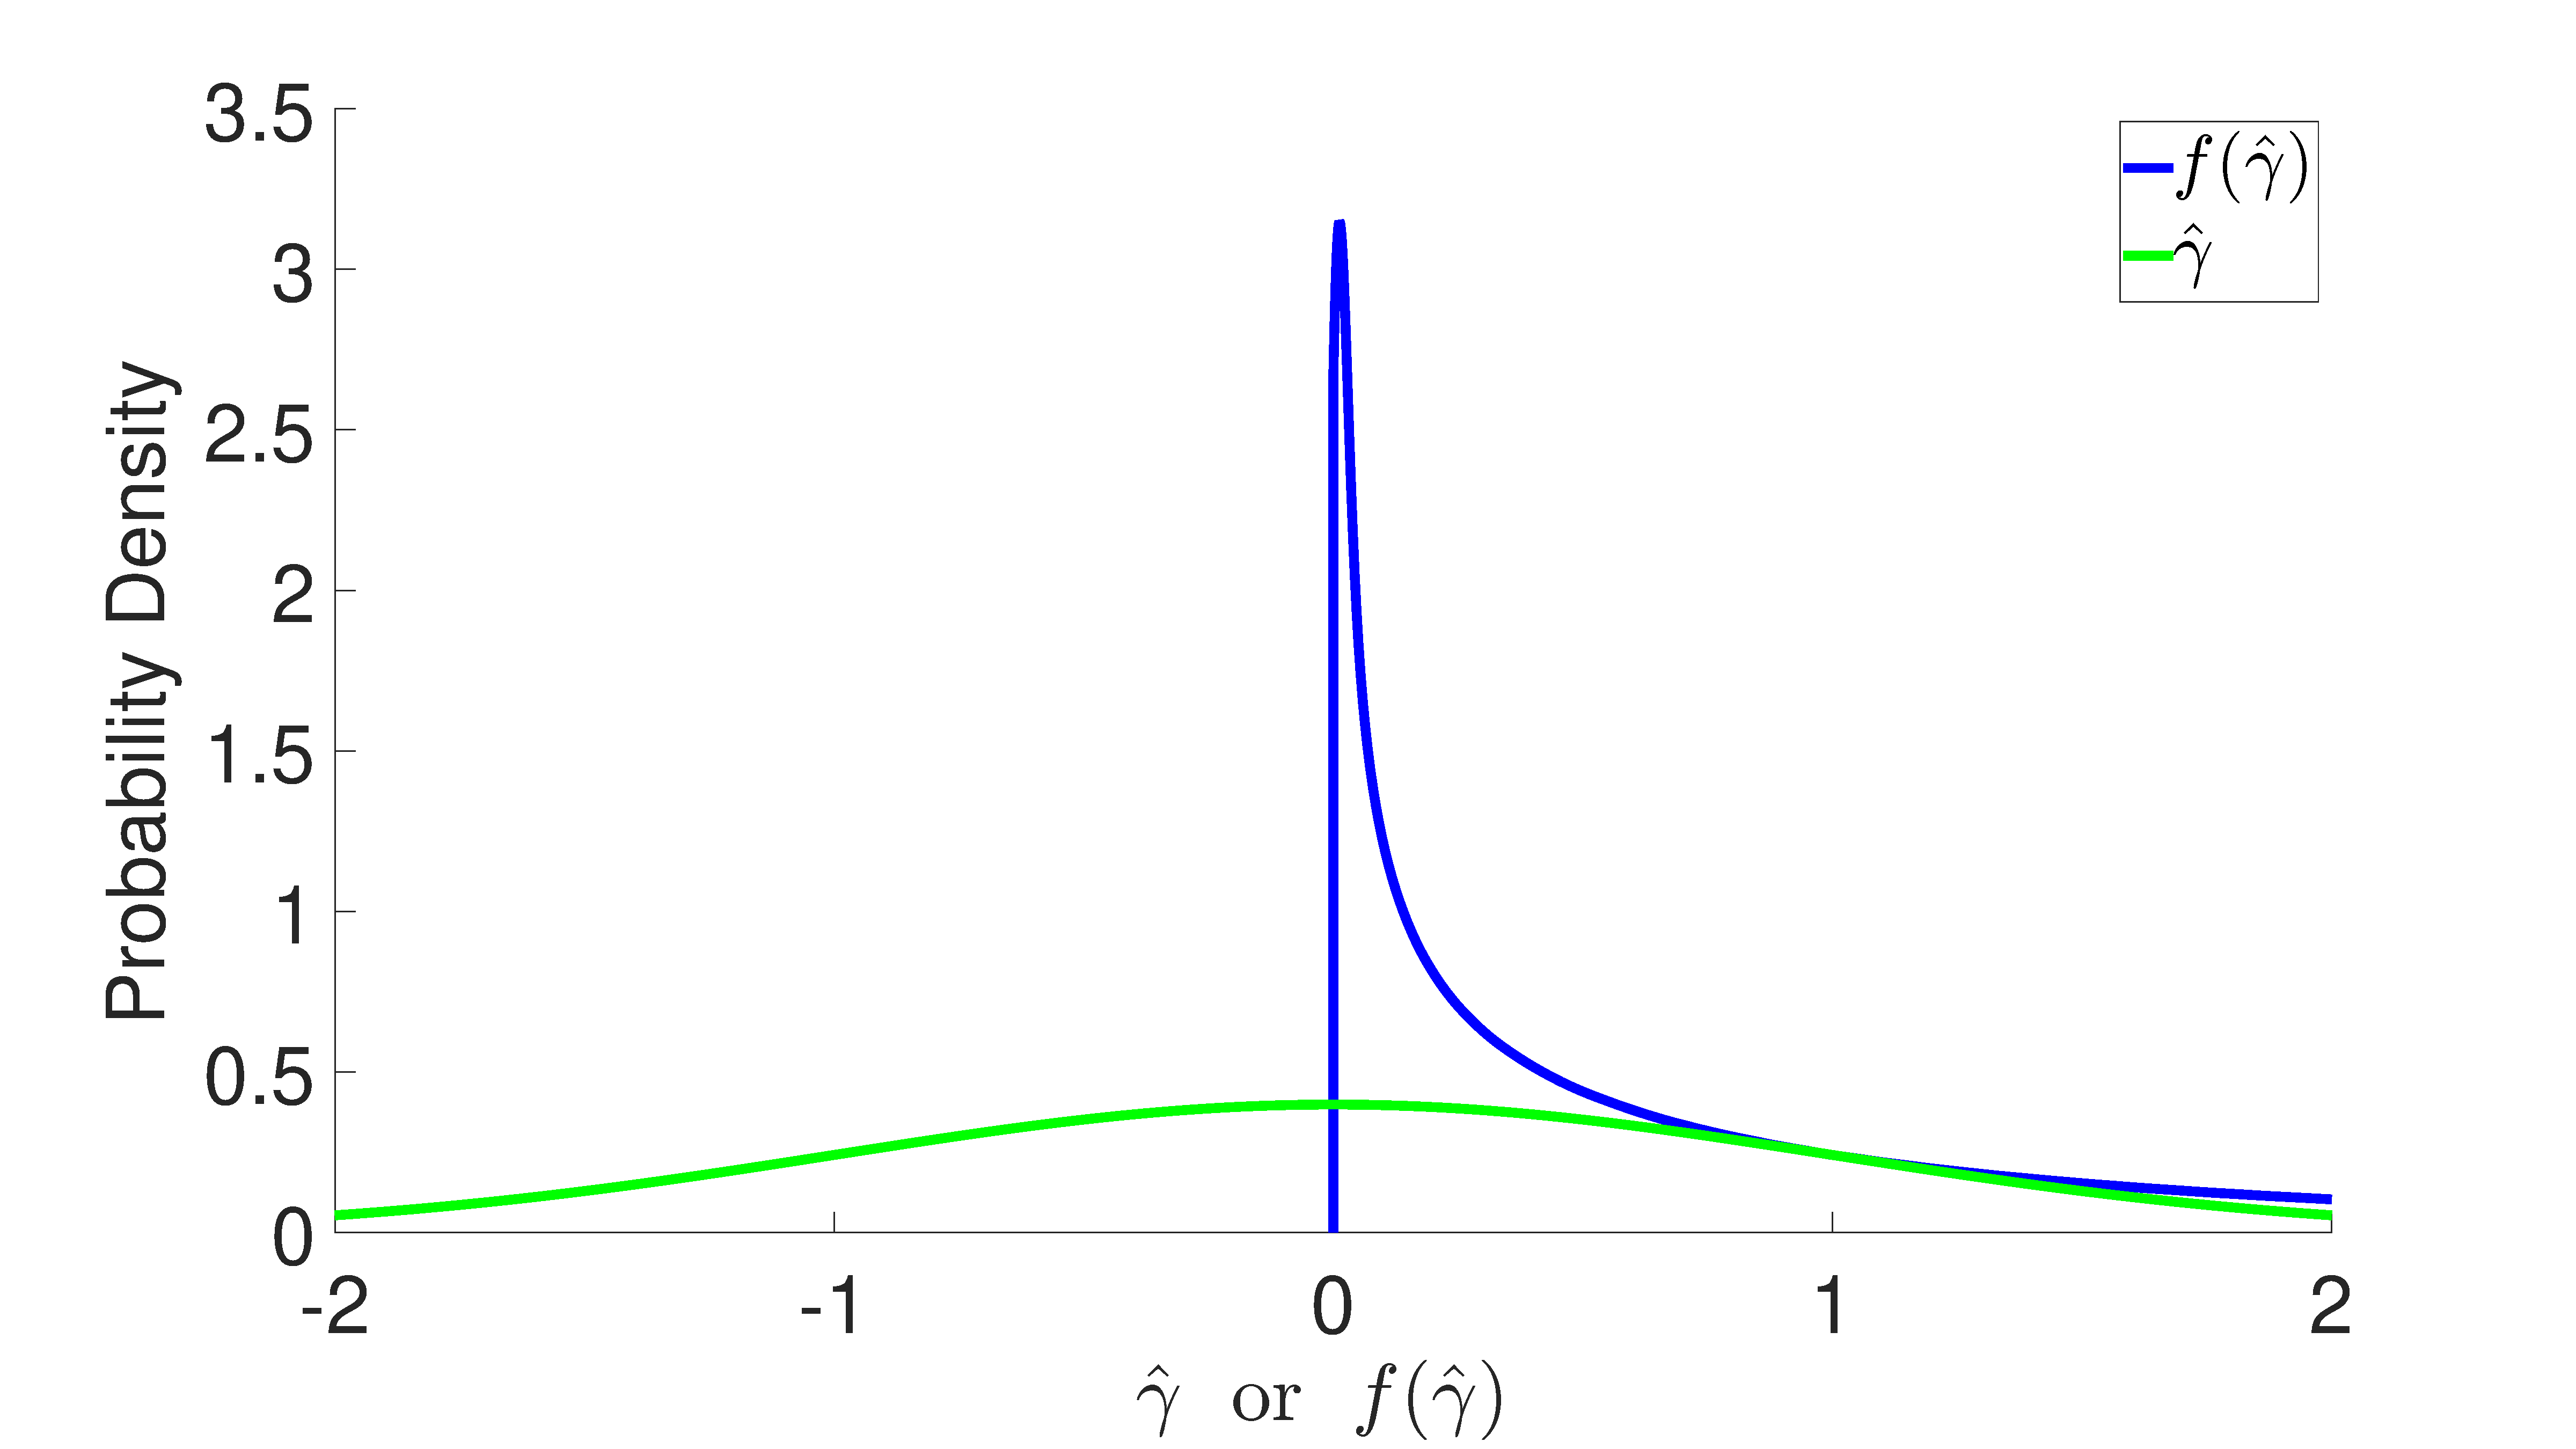
\includegraphics[width=0.5\textwidth]{bias_plot2}
%	\caption{Demonstration of inherent bias.  The true value of $\gamma(y)$ is taken as $0$ for all values of $y$.  Realisations for $\hg$, shown in green, are unbiased and distributed according to a unit Gaussian.  Shown in blue is the distribution of realisation of $f(\hg) = \hg^2$. All instances of $f(\hg)$ are positive and so $\E[f(\hg)]= 1 > 0 = f(\E[\hg])$.  Note also that the function $f'(\hg) = -\hg^2$ would have the opposite bias and so a simple bias correction is not possible.\label{fig:bias-plot}}
%\end{figure}
We now show that 
\emph{any}
strictly convex or concave $f$ entails a biased estimator 
when $\hat{\zeta}_n$ is unbiased but has non-zero variance
given $y_n$. This covers the
case where $\hat{\zeta}_n$ is a MC estimate.
\begin{theorem}
  \label{the:bias-conv}	
  Suppose that $y_n \sim p(y)$ and that each $\hat{\zeta}_n$ satisfies $\E \left[\hat{\zeta}_n \middle| y_n\right] = \gamma(y_n)$.
  Define $\mathcal{A} \subseteq \mathcal{Y}$ as
  $\mathcal{A} = \left\{y \in \mathcal{Y} \;\middle|\; \mathrm{Var}\left(\hat{\zeta}_n \middle| y_n=y \right)>0\right\}$
  and assume that ~$\mathbb{P}(y_n \in \mathcal{A}) > 0$.
  Then for any $f$ that is strictly convex in its second argument,
	$\E\left[\frac{1}{N} \sum_{n=1}^N f(y_n, \hat{\zeta}_n)\right] > I(f)$.
  Similarly for any $f$ that is strictly concave in its second argument, 
		$\E\left[\frac{1}{N} \sum_{n=1}^N f(y_n, \hat{\zeta}_n)\right] < I(f)$.
\end{theorem}
\begin{proof}
	If $f$ is strictly convex (the concave case follows by the same argument) we have
	\begin{align*}
	\E\left[\frac{1}{N} \sum_{n=1}^N f(y_n, \hat{\zeta}_n)\right] = \E\left[f(y_1, \hat{\zeta}_1)\right] 
	= \E\left[\E\left[f(y_1, \hat{\zeta}_1) \middle| y_1\right]\right] 
	\ge \E\left[f\left(y_1, \E\left[\hat{\zeta}_1 \middle| y_1\right]\right)\right] = I(f)
	%        \E&\left[\frac{1}{N} \sum_{n=1}^N f(y_n, \hat{\zeta}_n)\right] = \E\left[f(y_1, \hat{\zeta}_1)\right] \\
	%        & \quad \quad \quad \quad = \E\left[\E\left[f(y_1, \hat{\zeta}_1)|y_1\right]\right] \\
	%        & \quad \quad \quad \quad = \E\left[\mathbb{I}(y_1 \in \mathcal{A}) \E\left[f(y_1, \hat{\zeta}_1)|y_1\right]\right] \\
	%        & \quad \quad \quad \quad \quad + \E\left[\mathbb{I}(y_1 \notin \mathcal{A}) \E\left[f(y_1, \hat{\zeta}_1)|y_1\right]\right] \\
	%        & \quad \quad \quad \quad \ge \E\left[\mathbb{I}(y_1 \in \mathcal{A}) f\left(y_1, \E\left[\hat{\zeta}_1 \middle| y_1\right]\right)\right] \\
	%        & \quad \quad \quad \quad \quad + \E\left[\mathbb{I}(y_1 \notin \mathcal{A}) \E\left[f(y_1, \hat{\zeta}_1)|y_1\right]\right] \\    
	%        & \quad \quad \quad \quad = \E\left[\E\left[f(y_1, \hat{\zeta}_1)|y_1\right]\right] = I(f)
	\end{align*}
	where the $\ge$ is a result of Jensen's inequality on the inner expectation.  
	Since $f$ is strictly convex and therefore nonlinear, equality holds if and only if
	$\hat{\zeta}_1$ is almost surely constant given $y_1$. 
	This is violated whenever $y_1 \in \mathcal{A}$, which by assumption
	has a non-zero probability of occurring.  Consequently,
	the inequality must be strict, giving the desired result.
\end{proof}
For certain nonlinear $f$, it may still be possible to develop unbiased estimation
schemes using Russian roulette sampling~\citep{lyne2015russian} or other debiasing techniques.  
However, this induces its own complications: for some problems the resultant estimates
have infinite variance \citep{lyne2015russian} and as shown by \cite{jacob2015nonnegative}, there are 
no general purpose ``$f$-factories'' that produce both non-negative and
unbiased estimates for non-constant, positive output functions $f : \real \rightarrow \real^+$,
given unbiased estimates for the inputs.

%This result suggests that general purpose, unbiased inference is impossible for nested
%probabilistic program queries which cannot be mathematically expressed as single inference
%of the form~\eqref{eq:MC}.  Such rearrangement is not possible when the outer query
%depends nonlinearly on a \emph{marginal} of the inner query.  Consequently, query nesting
%using existing systems\footnote{We note that for certain nonlinear $f$, it may still be
%possible to develop an unbiased inference scheme using a combination of a convergent
%Maclaurin expansion and Russian Roulette sampling \cite{lyne2015russian}.} cannot provide
%unbiased estimation of problems that cannot be expressed as a single query.  However, the
%additional models that it does allow expression for, such as the experimental design
%example, might still be estimable in consistent fashion as shown in the previous section.
